% Readout taxonomy for typed decision models: where does the per-option score come from?
\documentclass[tikz,border=12pt]{standalone}
\usepackage{amsmath}
\usepackage{amssymb}
\usetikzlibrary{arrows.meta,positioning,calc,decorations.pathreplacing}

\definecolor{frozenfill}{HTML}{F3F4F6}
\definecolor{frozendraw}{HTML}{6B7280}
\definecolor{trainfill}{HTML}{EFF6FF}
\definecolor{trainraw}{HTML}{2563EB}
\definecolor{datafill}{HTML}{F0FDF4}
\definecolor{datadraw}{HTML}{16A34A}
\definecolor{markerfill}{HTML}{FEF2F2}
\definecolor{vocabfill}{HTML}{FFF7ED}
\definecolor{vocabdraw}{HTML}{EA580C}
\definecolor{codefill}{HTML}{F5F3FF}
\definecolor{codedraw}{HTML}{7C3AED}
\definecolor{markerdraw}{HTML}{DC2626}

\tikzset{
  panel/.style={draw=black!20, line width=0.5pt, rounded corners=4pt, fill=white},
  tok/.style={draw=black!45, fill=white, rounded corners=1.2pt,
              minimum height=0.40cm, inner sep=2.2pt, font=\sffamily\scriptsize},
  pgtok/.style={tok, fill=frozenfill, draw=frozendraw},
  opttok/.style={tok, fill=datafill, draw=datadraw},
  readtok/.style={tok, fill=markerfill, draw=markerdraw, font=\sffamily\scriptsize\bfseries},
  blanktok/.style={tok, dashed, fill=white},
  hbox/.style={draw=frozendraw, fill=frozenfill, rounded corners=2pt,
               minimum height=0.44cm, inner sep=2.5pt, font=\sffamily\scriptsize},
  trainbox/.style={draw=trainraw, fill=trainfill, rounded corners=2pt,
                   minimum height=0.44cm, inner sep=3pt, font=\sffamily\scriptsize,
                   align=center},
  vocabbox/.style={draw=vocabdraw, fill=vocabfill, rounded corners=2pt,
                   minimum height=0.44cm, inner sep=3pt, font=\sffamily\scriptsize,
                   align=center},
  code/.style={tok, fill=codefill, draw=codedraw, font=\sffamily\tiny\bfseries, inner xsep=1.8pt},
  bar/.style={draw=black!45, fill=black!12, minimum height=0.32cm,
              minimum width=0.60cm, font=\sffamily\tiny},
  arrow/.style={-{Stealth[length=1.8mm,width=1.4mm]}, line width=0.5pt, draw=black!70},
  darrow/.style={arrow, dashed},
  lbl/.style={font=\sffamily\tiny, text=black!65, align=center},
  note/.style={font=\sffamily\tiny, text=black!70, align=center},
  ttl/.style={font=\sffamily\small\bfseries, text=black!88, align=center},
  tag/.style={font=\sffamily\tiny, text=black!55, align=center},
}

\begin{document}
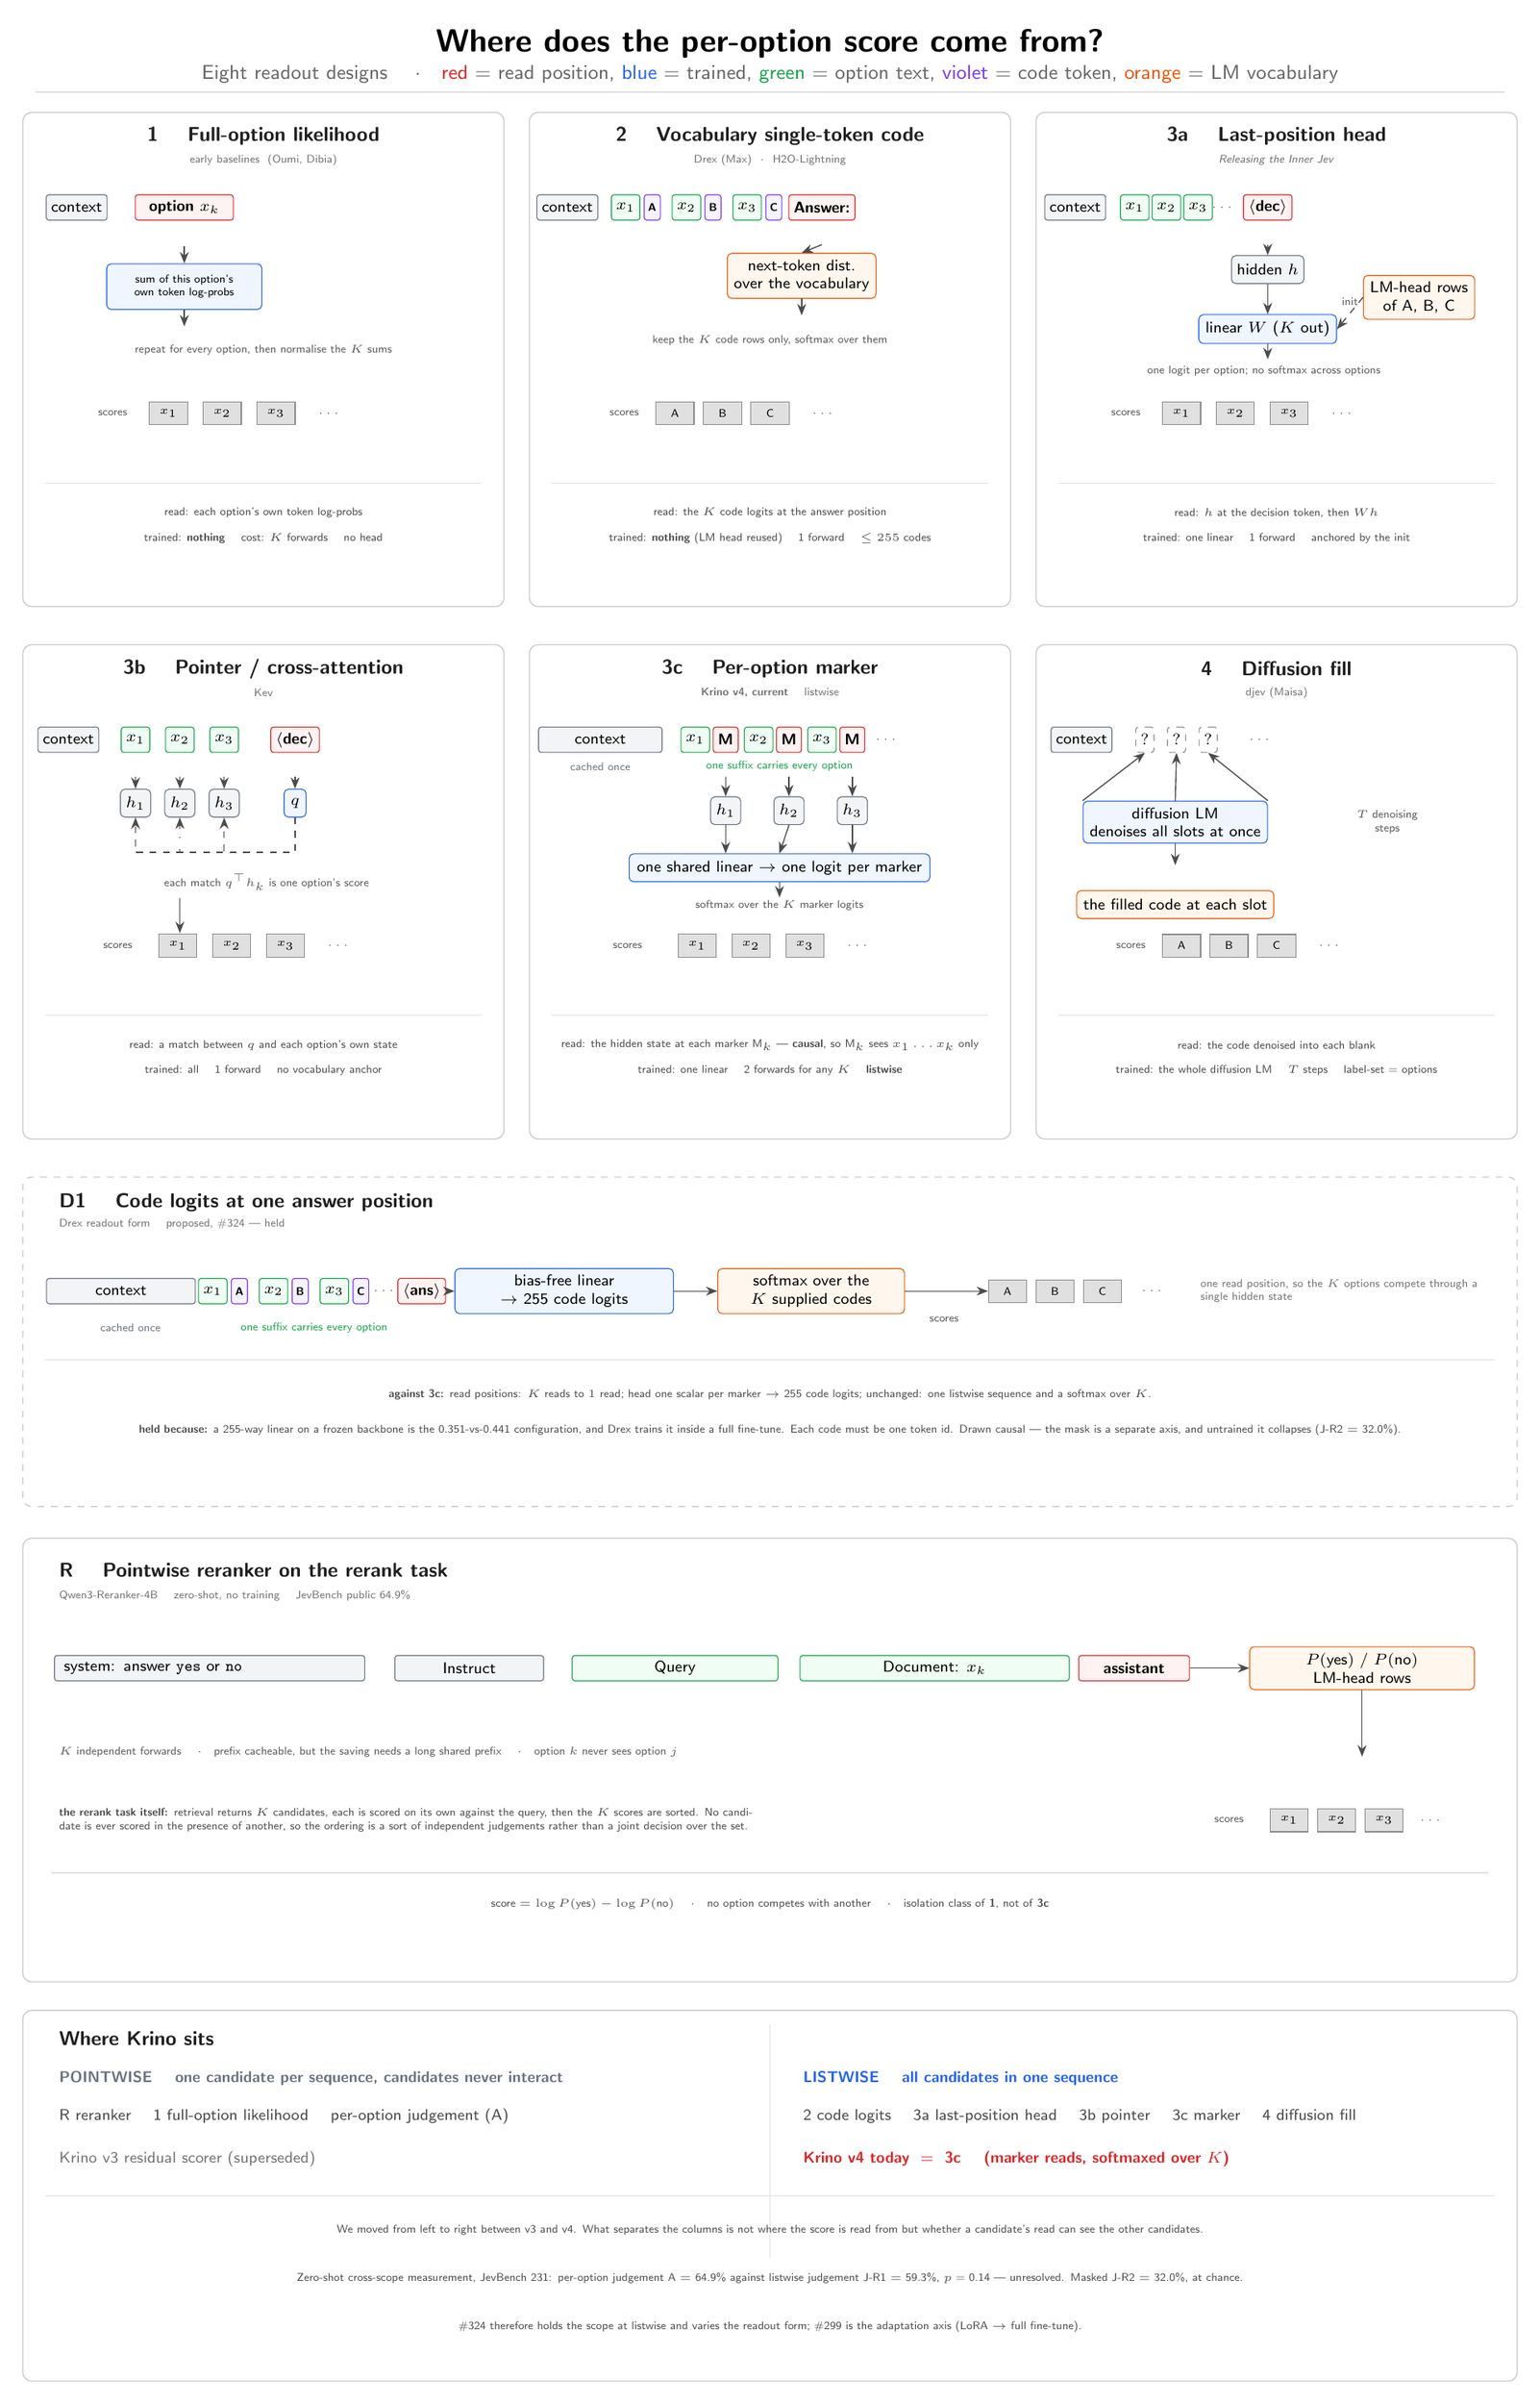
\begin{tikzpicture}[font=\sffamily]

\node[font=\sffamily\Large\bfseries] at (11.8,25.08)
  {Where does the per-option score come from?};
\node[font=\sffamily\small, text=black!60] at (11.8,24.60)
  {Eight readout designs \quad$\cdot$\quad \textcolor{markerdraw}{red} = read position, \textcolor{trainraw}{blue} = trained, \textcolor{datadraw}{green} = option text, \textcolor{codedraw}{violet} = code token, \textcolor{vocabdraw}{orange} = LM vocabulary};
\draw[black!20, line width=0.5pt] (0.2,24.32) -- (23.4,24.32);

% ================================================================ 1
\begin{scope}[shift={(0,16.2)}]
  \draw[panel] (0,0) rectangle (7.6,7.8);
  \node[ttl] at (3.8,7.42) {1 \quad Full-option likelihood};
  \node[tag] at (3.8,7.04) {early baselines \ (Oumi, Dibia)};

  \node[pgtok] (p1) at (0.85,6.30) {context};
  \node[readtok, minimum width=1.55cm] (o1) at (2.55,6.30) {option $x_k$};

  \node[trainbox, minimum width=2.45cm, minimum height=0.72cm,
        font=\sffamily\tiny, text width=2.15cm] (s1) at (2.55,5.05)
    {sum of this option's\\own token log-probs};
  \draw[arrow] ([yshift=-0.40cm]o1.south) -- (s1.north);

  \node[lbl, text width=6.4cm] at (3.80,4.05) {repeat for every option, then normalise the $K$ sums};
  \draw[arrow] (s1.south) -- ++(0,-0.26);

  \node[lbl] at (1.42,3.05) {scores};
  \node[bar] at (2.30,3.05) {$x_1$};
  \node[bar] at (3.15,3.05) {$x_2$};
  \node[bar] at (4.00,3.05) {$x_3$};
  \node[lbl] at (4.85,3.05) {$\cdots$};

  \draw[black!12, line width=0.5pt] (0.35,1.95) -- (7.25,1.95);
  \node[note] at (3.8,1.48) {read: each option's own token log-probs};
  \node[note] at (3.8,1.08) {trained: \textbf{nothing} \quad cost: $K$ forwards \quad no head};
\end{scope}

% ================================================================ 2
\begin{scope}[shift={(8.0,16.2)}]
  \draw[panel] (0,0) rectangle (7.6,7.8);
  \node[ttl] at (3.8,7.42) {2 \quad Vocabulary single-token code};
  \node[tag] at (3.8,7.04) {Drex (Max) \ $\cdot$ \ H2O-Lightning};

  \node[pgtok] (p2) at (0.60,6.30) {context};
  \node[opttok] (c2x1) at (1.52,6.30) {$x_1$};
  \node[code]   (c2a)  at (1.94,6.30) {A};
  \node[opttok] (c2x2) at (2.48,6.30) {$x_2$};
  \node[code]   (c2b)  at (2.90,6.30) {B};
  \node[opttok] (c2x3) at (3.44,6.30) {$x_3$};
  \node[code]   (c2c)  at (3.86,6.30) {C};
  \node[readtok] (a2) at (4.62,6.30) {Answer:};

  \node[vocabbox, minimum width=2.05cm] (v2) at (4.30,5.22)
    {next-token dist.\\over the vocabulary};
  \draw[arrow] ([yshift=-0.38cm]a2.south) -- (v2.north);

  \node[lbl, text width=6.4cm] at (3.80,4.20) {keep the $K$ code rows only, softmax over them};
  \draw[arrow] (v2.south) -- ++(0,-0.26);

  \node[lbl] at (1.50,3.05) {scores};
  \node[bar] at (2.30,3.05) {A};
  \node[bar] at (3.05,3.05) {B};
  \node[bar] at (3.80,3.05) {C};
  \node[lbl] at (4.65,3.05) {$\cdots$};

  \draw[black!12, line width=0.5pt] (0.35,1.95) -- (7.25,1.95);
  \node[note] at (3.8,1.48) {read: the $K$ code logits at the answer position};
  \node[note] at (3.8,1.08) {trained: \textbf{nothing} (LM head reused) \quad 1 forward \quad $\le 255$ codes};
\end{scope}

% ================================================================ 3a
\begin{scope}[shift={(16.0,16.2)}]
  \draw[panel] (0,0) rectangle (7.6,7.8);
  \node[ttl] at (3.8,7.42) {3a \quad Last-position head};
  \node[tag] at (3.8,7.04) {\emph{Releasing the Inner Jev}};

  \node[pgtok] (p3) at (0.62,6.30) {context};
  \node[opttok] (x31) at (1.56,6.30) {$x_1$};
  \node[opttok] (x32) at (2.06,6.30) {$x_2$};
  \node[opttok] (x33) at (2.56,6.30) {$x_3$};
  \node[lbl] at (2.96,6.30) {$\cdots$};
  \node[readtok] (d3) at (3.66,6.30) {$\langle$dec$\rangle$};

  \node[hbox] (h3) at (3.66,5.32) {hidden $h$};
  \draw[arrow] ([yshift=-0.38cm]d3.south) -- (h3.north);

  \node[trainbox, minimum width=1.95cm] (w3) at (3.66,4.38) {linear $W$ ($K$ out)};
  \draw[arrow] (h3.south) -- (w3.north);

  \node[vocabbox, minimum width=1.65cm] (i3) at (6.05,4.88) {LM-head rows\\of A, B, C};
  \draw[darrow] (i3.west) -- node[above, lbl] {init} (w3.east);

  \node[lbl, text width=6.4cm] at (3.60,3.72) {one logit per option; no softmax across options};
  \draw[arrow] (w3.south) -- ++(0,-0.24);

  \node[lbl] at (1.42,3.05) {scores};
  \node[bar] at (2.30,3.05) {$x_1$};
  \node[bar] at (3.15,3.05) {$x_2$};
  \node[bar] at (4.00,3.05) {$x_3$};
  \node[lbl] at (4.85,3.05) {$\cdots$};

  \draw[black!12, line width=0.5pt] (0.35,1.95) -- (7.25,1.95);
  \node[note] at (3.8,1.48) {read: $h$ at the decision token, then $Wh$};
  \node[note] at (3.8,1.08) {trained: one linear \quad 1 forward \quad anchored by the init};
\end{scope}

% ================================================================ 3b
\begin{scope}[shift={(0,7.8)}]
  \draw[panel] (0,0) rectangle (7.6,7.8);
  \node[ttl] at (3.8,7.42) {3b \quad Pointer / cross-attention};
  \node[tag] at (3.8,7.04) {Kev};

  \node[pgtok] (p4) at (0.72,6.30) {context};
  \node[opttok] (x41) at (1.78,6.30) {$x_1$};
  \node[opttok] (x42) at (2.48,6.30) {$x_2$};
  \node[opttok] (x43) at (3.18,6.30) {$x_3$};
  \node[readtok] (q4) at (4.30,6.30) {$\langle$dec$\rangle$};

  \node[hbox] (h41) at (1.78,5.30) {$h_1$};
  \node[hbox] (h42) at (2.48,5.30) {$h_2$};
  \node[hbox] (h43) at (3.18,5.30) {$h_3$};
  \node[trainbox] (q4b) at (4.30,5.30) {$q$};
  \draw[arrow] ([yshift=-0.38cm]q4.south) -- (q4b.north);
  \draw[arrow] ([yshift=-0.38cm]x41.south) -- (h41.north);
  \draw[arrow] ([yshift=-0.38cm]x42.south) -- (h42.north);
  \draw[arrow] ([yshift=-0.38cm]x43.south) -- (h43.north);

  \draw[darrow] (q4b.south) -- ++(0,-0.55) -| (h41.south);
  \draw[darrow] (q4b.south) -- ++(0,-0.55) -| (h42.south);
  \draw[darrow] (q4b.south) -- ++(0,-0.55) -| (h43.south);
  \node[lbl, fill=white, inner sep=1pt] at (2.48,4.75) {$\cdot$};

  \node[lbl, text width=6.3cm] at (3.85,4.05)
    {each match $q^{\top}h_k$ is one option's score};
  \draw[arrow] (2.48,3.80) -- ++(0,-0.55);

  \node[lbl] at (1.50,3.05) {scores};
  \node[bar] at (2.45,3.05) {$x_1$};
  \node[bar] at (3.30,3.05) {$x_2$};
  \node[bar] at (4.15,3.05) {$x_3$};
  \node[lbl] at (5.00,3.05) {$\cdots$};

  \draw[black!12, line width=0.5pt] (0.35,1.95) -- (7.25,1.95);
  \node[note] at (3.8,1.48) {read: a match between $q$ and each option's own state};
  \node[note] at (3.8,1.08) {trained: all \quad 1 forward \quad no vocabulary anchor};
\end{scope}

% ================================================================ 3c  (LISTWISE)
\begin{scope}[shift={(8.0,7.8)}]
  \draw[panel] (0,0) rectangle (7.6,7.8);
  \node[ttl] at (3.8,7.42) {3c \quad Per-option marker};
  \node[tag] at (3.8,7.04) {\textbf{Krino v4, current} \quad listwise};

  \node[pgtok, minimum width=1.95cm] (s3) at (1.12,6.30) {context};
  \node[opttok] (a3) at (2.62,6.30) {$x_1$};
  \node[readtok] (m3) at (3.10,6.30) {M};
  \node[opttok] (b3) at (3.62,6.30) {$x_2$};
  \node[readtok] (n3) at (4.10,6.30) {M};
  \node[opttok] (c3) at (4.62,6.30) {$x_3$};
  \node[readtok] (p3) at (5.10,6.30) {M};
  \node[lbl] at (5.65,6.30) {$\cdots$};

  \node[font=\sffamily\tiny, text=frozendraw] at (1.12,5.88) {cached once};
  \node[font=\sffamily\tiny, text=datadraw] at (3.95,5.88) {one suffix carries every option};

  \node[hbox] (h31) at (3.10,5.18) {$h_1$};
  \node[hbox] (h32) at (4.10,5.18) {$h_2$};
  \node[hbox] (h33) at (5.10,5.18) {$h_3$};
  \draw[arrow] ([yshift=-0.38cm]m3.south) -- (h31.north);
  \draw[arrow] ([yshift=-0.38cm]n3.south) -- (h32.north);
  \draw[arrow] ([yshift=-0.38cm]p3.south) -- (h33.north);

  \node[trainbox, minimum width=4.75cm] (mh) at (3.95,4.28)
    {one shared linear $\rightarrow$ one logit per marker};
  \draw[arrow] (h31.south) -- (h31.south |- mh.north);
  \draw[arrow] (h32.south) -- (mh.north);
  \draw[arrow] (h33.south) -- (h33.south |- mh.north);

  \node[lbl] at (3.95,3.68) {softmax over the $K$ marker logits};
  \draw[arrow] (mh.south) -- ++(0,-0.24);

  \node[lbl] at (1.55,3.05) {scores};
  \node[bar] at (2.65,3.05) {$x_1$};
  \node[bar] at (3.50,3.05) {$x_2$};
  \node[bar] at (4.35,3.05) {$x_3$};
  \node[lbl] at (5.20,3.05) {$\cdots$};

  \draw[black!12, line width=0.5pt] (0.35,1.95) -- (7.25,1.95);
  \node[note] at (3.8,1.48) {read: the hidden state at each marker M$_k$ --- \textbf{causal}, so M$_k$ sees $x_1\ldots x_k$ only};
  \node[note] at (3.8,1.08) {trained: one linear \quad 2 forwards for any $K$ \quad \textbf{listwise}};
\end{scope}

% ================================================================ 4
\begin{scope}[shift={(16.0,7.8)}]
  \draw[panel] (0,0) rectangle (7.6,7.8);
  \node[ttl] at (3.8,7.42) {4 \quad Diffusion fill};
  \node[tag] at (3.8,7.04) {djev (Maisa)};

  \node[pgtok] (p6) at (0.72,6.30) {context};
  \node[blanktok] (z61) at (1.72,6.30) {$?$};
  \node[blanktok] (z62) at (2.22,6.30) {$?$};
  \node[blanktok] (z63) at (2.72,6.30) {$?$};
  \node[lbl] at (3.55,6.30) {$\cdots$};

  \node[trainbox, minimum width=2.35cm] (dlm) at (2.20,5.00)
    {diffusion LM\\denoises all slots at once};
  \draw[arrow] (dlm.north west) -- (z61.south);
  \draw[arrow] (dlm.north) -- (z62.south);
  \draw[arrow] (dlm.north east) -- (z63.south);

  \node[lbl, text width=2.6cm] at (5.55,5.00) {$T$ denoising\\steps};
  \draw[arrow] (dlm.south) -- ++(0,-0.34);

  \node[vocabbox, minimum width=2.1cm] (o6) at (2.20,3.70) {the filled code at each slot};

  \node[lbl] at (1.50,3.05) {scores};
  \node[bar] at (2.30,3.05) {A};
  \node[bar] at (3.05,3.05) {B};
  \node[bar] at (3.80,3.05) {C};
  \node[lbl] at (4.65,3.05) {$\cdots$};

  \draw[black!12, line width=0.5pt] (0.35,1.95) -- (7.25,1.95);
  \node[note] at (3.8,1.48) {read: the code denoised into each blank};
  \node[note] at (3.8,1.08) {trained: the whole diffusion LM \quad $T$ steps \quad label-set = options};
\end{scope}

% ================================================================ D1 (proposed)
\begin{scope}[shift={(0,2.00)}]
  \draw[panel, dashed] (0,0) rectangle (23.6,5.2);

  \node[anchor=west, font=\sffamily\small\bfseries, text=black!88] at (0.45,4.80)
    {D1 \quad Code logits at one answer position};
  \node[anchor=west, tag] at (0.45,4.45)
    {Drex readout form \quad proposed, \#324 --- held};

  \node[pgtok, minimum width=2.35cm] (d1p) at (1.55,3.40) {context};
  \node[opttok] (d1a) at (3.00,3.40) {$x_1$};
  \node[code]   (d1ca) at (3.42,3.40) {A};
  \node[opttok] (d1b) at (3.96,3.40) {$x_2$};
  \node[code]   (d1cb) at (4.38,3.40) {B};
  \node[opttok] (d1c) at (4.92,3.40) {$x_3$};
  \node[code]   (d1cc) at (5.34,3.40) {C};
  \node[lbl] at (5.72,3.40) {$\cdots$};
  \node[readtok] (d1q) at (6.30,3.40) {$\langle$ans$\rangle$};

  \node[font=\sffamily\tiny, text=frozendraw] at (1.70,2.82) {cached once};
  \node[font=\sffamily\tiny, text=datadraw] at (4.60,2.82) {one suffix carries every option};

  \node[trainbox, minimum width=3.45cm] (d1w) at (8.55,3.40)
    {bias-free linear\\$\rightarrow$ 255 code logits};
  \draw[arrow] (d1q.east) -- (d1w.west);

  \node[vocabbox, minimum width=2.95cm] (d1s) at (12.45,3.40)
    {softmax over the\\$K$ supplied codes};
  \draw[arrow] (d1w.east) -- (d1s.west);

  \node[bar] (d1b1) at (15.55,3.40) {A};
  \node[bar] (d1b2) at (16.30,3.40) {B};
  \node[bar] (d1b3) at (17.05,3.40) {C};
  \node[lbl] at (17.85,3.40) {$\cdots$};
  \node[lbl] at (14.55,2.95) {scores};
  \draw[arrow] (d1s.east) -- (d1b1.west);

  \node[font=\sffamily\tiny, text=black!55, align=left, text width=4.6cm] at (20.9,3.40)
    {one read position, so the $K$ options compete through a single hidden state};

  \draw[black!12, line width=0.5pt] (0.35,2.32) -- (23.25,2.32);
  \node[note, text width=22.6cm, align=center] at (11.8,1.76)
    {\textbf{against 3c:} read positions: $K$ reads to $1$ read; head one scalar per marker $\rightarrow$ 255 code logits; unchanged: one listwise sequence and a softmax over $K$.};
  \node[note, text width=22.6cm, align=center] at (11.8,1.20)
    {\textbf{held because:} a 255-way linear on a frozen backbone is the 0.351-vs-0.441 configuration, and Drex trains it inside a full fine-tune. Each code must be one token id. Drawn causal --- the mask is a separate axis, and untrained it collapses (J-R2 $=$ 32.0\%).};
\end{scope}

% ================================================================ R (baseline)
\begin{scope}[shift={(0,-5.50)}]
  \draw[panel] (0,0) rectangle (23.6,7.0);

  \node[anchor=west, font=\sffamily\small\bfseries, text=black!88] at (0.45,6.50)
    {R \quad Pointwise reranker on the rerank task};
  \node[anchor=west, tag] at (0.45,6.10)
    {Qwen3-Reranker-4B \quad zero-shot, no training \quad JevBench public 64.9\%};

  \node[pgtok, minimum width=4.9cm, text width=4.6cm] (rsys) at (2.95,4.95)
    {system: answer \texttt{yes} or \texttt{no}};
  \node[pgtok, minimum width=2.35cm] (rins) at (7.05,4.95) {Instruct};
  \node[opttok, minimum width=3.25cm] (rq) at (10.30,4.95) {Query};
  \node[opttok, minimum width=4.25cm] (rd) at (14.40,4.95) {Document: $x_k$};
  \node[readtok, minimum width=1.75cm] (ra) at (17.55,4.95) {assistant};

  \node[vocabbox, minimum width=3.55cm, minimum height=0.62cm] (rv) at (21.15,4.95)
    {$P(\text{yes})$ / $P(\text{no})$\\LM-head rows};
  \draw[arrow] (ra.east) -- (rv.west);

  \node[lbl, anchor=west] at (0.45,3.62)
    {$K$ independent forwards \quad$\cdot$\quad prefix cacheable, but the saving needs a long shared prefix \quad$\cdot$\quad option $k$ never sees option $j$};

  \draw[arrow] (rv.south) -- ++(0,-1.05);

  \node[note, anchor=west, text width=11.2cm, align=left] at (0.45,2.55)
    {\hyphenpenalty=10000\exhyphenpenalty=10000\textbf{the rerank task itself:} retrieval returns $K$ candidates, each is scored on its own against the query, then the $K$ scores are sorted. No candidate is ever scored in the presence of another, so the ordering is a sort of independent judgements rather than a joint decision over the set.};

  \node[lbl] at (19.05,2.55) {scores};
  \node[bar] at (20.00,2.55) {$x_1$};
  \node[bar] at (20.75,2.55) {$x_2$};
  \node[bar] at (21.50,2.55) {$x_3$};
  \node[lbl] at (22.25,2.55) {$\cdots$};

  \draw[black!12, line width=0.5pt] (0.45,1.72) -- (23.15,1.72);
  \node[note] at (11.8,1.22)
    {score $=\log P(\text{yes})-\log P(\text{no})$ \quad$\cdot$\quad no option competes with another \quad$\cdot$\quad isolation class of \textbf{1}, not of \textbf{3c}};
\end{scope}

% ================================================================ positioning
\begin{scope}[shift={(0,-11.80)}]
  \draw[panel] (0,0) rectangle (23.6,5.85);

  \node[anchor=west, font=\sffamily\small\bfseries, text=black!88] at (0.45,5.40)
    {Where Krino sits};
  \draw[black!12, line width=0.5pt] (11.80,1.95) -- (11.80,5.62);

  % ---- pointwise
  \node[anchor=west, font=\sffamily\scriptsize\bfseries, text=frozendraw] at (0.45,4.78)
    {POINTWISE \quad one candidate per sequence, candidates never interact};
  \node[anchor=west, font=\sffamily\scriptsize, text=black!72] at (0.45,4.18)
    {R reranker \quad 1 full-option likelihood \quad per-option judgement (A)};
  \node[anchor=west, font=\sffamily\scriptsize, text=black!55] at (0.45,3.50)
    {Krino v3 residual scorer (superseded)};

  % ---- listwise
  \node[anchor=west, font=\sffamily\scriptsize\bfseries, text=trainraw] at (12.20,4.78)
    {LISTWISE \quad all candidates in one sequence};
  \node[anchor=west, font=\sffamily\scriptsize, text=black!72] at (12.20,4.18)
    {2 code logits \quad 3a last-position head \quad 3b pointer \quad 3c marker \quad 4 diffusion fill};
  \node[anchor=west, font=\sffamily\scriptsize\bfseries, text=markerdraw] at (12.20,3.50)
    {Krino v4 today $\;=\;$ 3c \quad (marker reads, softmaxed over $K$)};

  \draw[black!12, line width=0.5pt] (0.35,2.92) -- (23.25,2.92);
  \node[note, text width=22.6cm, align=center] at (11.8,2.38)
    {We moved from left to right between v3 and v4. What separates the columns is not where the score is read from but whether a candidate's read can see the other candidates.};
  \node[note, text width=22.6cm, align=center] at (11.8,1.62)
    {Zero-shot cross-scope measurement, JevBench 231: per-option judgement A $=$ 64.9\% against listwise judgement J-R1 $=$ 59.3\%, $p$ = 0.14 --- unresolved. Masked J-R2 $=$ 32.0\%, at chance.};
  \node[note, text width=22.6cm, align=center] at (11.8,0.86)
    {\#324 therefore holds the scope at listwise and varies the readout form; \#299 is the adaptation axis (LoRA $\rightarrow$ full fine-tune).};
\end{scope}
\end{tikzpicture}
\end{document}
